
When the quench is generated, the point at which the cable transitions from the superconducting to the normal conducting state propagates over time, as shown in Fig. \ref{fig:quench_front_propagation_illustration}. This point remains at the critical temperature, $T_\text{c}$ for a given magnetic field strength and current density. The time derivative of the quench front position is referred to as quench velocity. At fixed current and magnetic field strength, the quench velocity remains constant.

\begin{figure}[H]
\centering
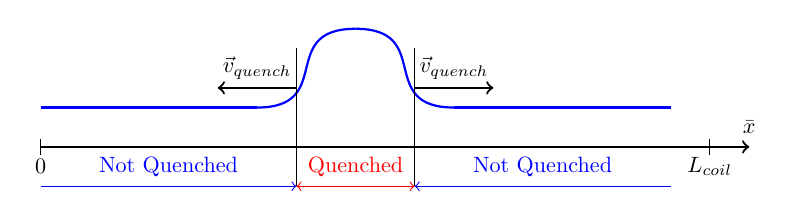
\begin{tikzpicture}[scale = 1]
\draw [thick, ->] (0.0,0.0) -- (9.0,0);

\draw [thick, blue] (0.0,0.5) -- (2.75,0.5);
\draw [thick, blue] (5.25,0.5) -- (8.0,0.5);

\draw [thick, blue] (2.75,0.5) .. controls +(0:1cm) and +(180:1cm) .. (4.0,1.5);
\draw [thick, blue] (4.0,1.5) .. controls +(0:1cm) and +(180:1cm) .. (5.25,0.5);

\draw [thin] (3.25,-0.5) -- (3.25,1.25);
\draw [thin] (4.75,-0.5) -- (4.75,1.25);

\draw [thick, ->] (4.75,0.75) -- (5.75,0.75);
\draw [thick, ->] (3.25,0.75) -- (2.25,0.75);

\draw [thin, red, <->] (3.25,-0.5) -- (4.75,-0.5);
\draw [thin, blue, ->] (0.0,-0.5) -- (3.25,-0.5);
\draw [thin, blue, <-] (4.75,-0.5) -- (8.0,-0.5);

\node[scale = 0.8] [color = red] at (4.0,-0.25) {Quenched};
\node[scale = 0.8] [color = blue] at (1.625,-0.25) {Not Quenched};
\node[scale = 0.8] [color = blue] at (6.375,-0.25) {Not Quenched};

\node[scale = 0.8] at (5.25,1.0) {$\vec{v}_\text{quench}$};
\node[scale = 0.8] at (2.75,1.0) {$\vec{v}_\text{quench}$};

\node[scale = 0.8] at (9.0,+0.25) {$\bar x$};
\node[scale = 0.8] at (8.5,-0.25) {$L_\text{coil}$};
\draw [thin] (8.5,-0.10) -- (8.5,0.10);
\draw [thin] (0,-0.10) -- (0,0.10);
\node[scale = 0.8] at (0,-0.25) {0};

\end{tikzpicture}
\caption{Schematic of dividing the coil length into the quenched and non-quenched zone.}
\label{fig:quench_front_propagation_illustration}
\end{figure}

Quench velocity can be approximated with analytic formulae. They are usually a function of current density, composite strand material properties and temperature gradient around the quench front. For superconducting accelerator magnets, Wilson's formula is often applied to estimate the quench velocity if cooling with liquid helium is not considered \cite[p.~206]{wilson1987superconducting}. In principle, it is possible to estimate the quench velocity in three different manners. It can be:
\begin{enumerate}
\item based on available measurements;
\item calculated analytically based on available formulae; or
\item calculated numerically based on a short numerical model with refined mesh to solve the quench front with sufficient precision (ideally validated against the measurements).
\end{enumerate}